\section{Umgesetzte Kompressionsverfahren} \label{konzept}
In diesem Abschnitt werden die einzelnen Verfahren vorgestellt. Im ersten Unterabschnitt \ref{konzept:ist-komprimierung} wird die Ist-Kompression analysiert. In den nächsten Unterabschnitten \ref{konzept:loesung0} bis \ref{konzept:prediktiv} werden die entwickelten Kompressionsverfahren und ihre Teilschritte vorgestellt.

\subsection{Ist-Kompression} \label{konzept:ist-komprimierung}
\begin{figure}[!htbp]
	\center
	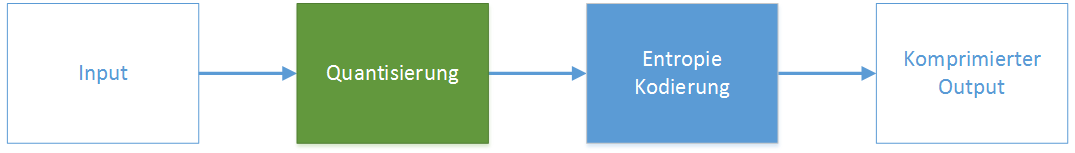
\includegraphics[width=0.8\textwidth,height=6cm,keepaspectratio]{./pictures/konzept/ist/aufbau.png}
	\caption{Aufbau der Ist-Kompression.}
	\label{konzept:ist:aufbau:diagramm}
\end{figure}
Das Ziel der Ist-Kompression ist es, die Datenmenge mit einfachen Mitteln zu reduzieren. Der Aufbau ist im Diagramm der Abbildung \ref{konzept:ist:aufbau:diagramm} dargestellt. Die Ist-Kompression führt zuerst ein Subsampling durch. Drei Viertel der Daten werden in diesem Schritt verworfen. Im Quantisierungsschritt werden die Daten von 32 Bit Floating Point auf 16-Bit Integer diskretisiert. In der Entropiekodierung werden die Daten geordnet wie in Tabelle \ref{konzept:ist:entropie} dargestellt.

\begin{table}[!htbp]
	\center
	\begin{tabular}{|c|c|c|c|}
	\hline
	Anzahl Punkte der Feldlinien & X Kanal aller Punkte & Y Kanal aller Punkte & Z Kanal aller Punkte \\\hline
	\end{tabular}
	\caption{Anordnung der Simulationsdaten der Ist-Kompression}
	\label{konzept:ist:entropie}
\end{table}
Als erstes werden die Längen aller Feldlinien abgelegt. Danach folgt der X, Y und der Z Kanal aller Punkte der Feldlinien. Diese Anordnung verbessert die Kompressionsrate der Entropiekodierung. Je näher ähnliche Muster beieinander liegen, desto besser können sie komprimiert werden. Für die eigentliche Entropie-Kodierung wird GZIP verwendet.\\
Die Datenmenge ist für eine performante Visualisierung zu gross. Um die Datenmenge für die zu verkleinern, wird nach der Übertragung ein Subsampling durchgeführt, das im Abschnitt \ref{konzept:loesung0:subsampling} beschrieben wird.

\subsection{Kompressionsverfahren: Adaptives Subsampling} \label{konzept:loesung0}
\begin{figure}[!htbp]
	\center
	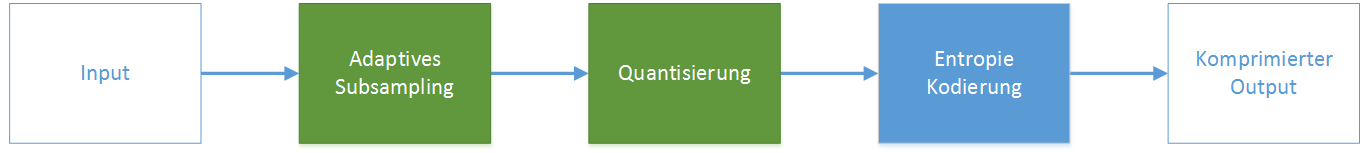
\includegraphics[width=0.8\textwidth,height=6cm,keepaspectratio]{./pictures/konzept/solution0/aufbau.png}
	\caption{Aufbau des Kompressionsvervahrens: Adaptives Subsampling.}
	\label{konzept:loesung0:aufbau:diagramm}
\end{figure} 
Dieses Verfahren verwendet einen ähnlichen Aufbau wie die Ist-Kompression. Der Unterschied ist, dass das Subsampling Verfahren gewählt wurde, welches der JHelioviewer vor der Visualisierung durchführt. Die Abbildung \ref{konzept:loesung0:aufbau:diagramm} zeigt den Ablauf dieses Verfahrens.\\

\subsubsection{Adaptives Subsampling}\label{konzept:loesung0:subsampling}
Konzeptionell approximiert das Adaptive Subsambling eine Punktfolge durch eine Folge von Strecken. Je stärker die Krümmung der Kurve, desto mehr Strecken wird für die Approximation benötigt.

\begin{figure}[!htbp]
	\center
	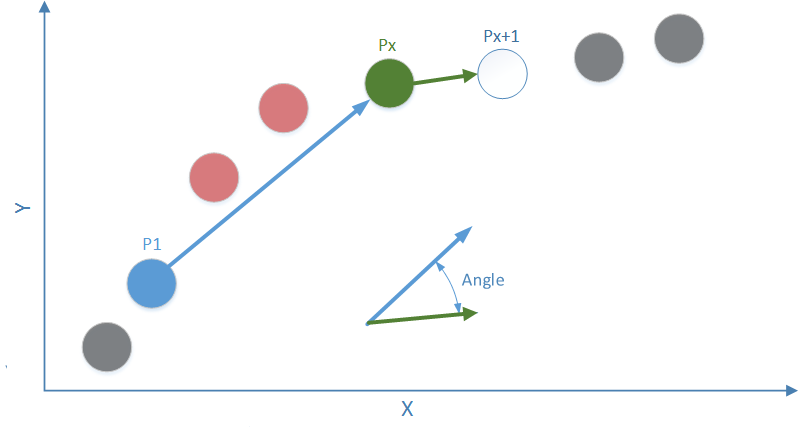
\includegraphics[width=0.8\textwidth,height=6cm,keepaspectratio]{./pictures/konzept/solution0/anglesubsampling.png}
	\caption{Darstellung des Adaptiven Subsapmlings. Rote Punkte wurden geprüft und gelöscht.}
	\label{konzept:loesung0:angle}
\end{figure}
Das Diagramm der Abbildung \ref{konzept:loesung0:angle} stellt das Subsampling im zweidimensionalen Raum dar. Das Adaptive Subsampling wählt nun Punkte $P$ aus der Feldlinie aus, welche Start- und Endpunkte der Strecken darstellen.\\
$P_1$ wurde bereits ausgewählt. Es wird nun ein Punkt $P_x$ gesucht, der als Endpunkt einer Strecke von $P_1$ zu $P_x$ die Daten approximiert. Dazu wird der Winkel der Strecke $P_1$ zu $P_x$ mit der Strecke $P_x$ zu $P_x+1$ verglichen. Wenn der Winkel kleiner ist, als ein Winkel $\alpha$, wird der nächste Punkt $P_x+1$ überprüft. Wenn der Winkel grösser ist, wird $P_x$ ausgewählt. Danach wird der wird eine nächste Strecke startend von $P_x$ gesucht.

\subsubsection{Entropiekodierung mittels RAR} \label{konzept:loesung0:kodierung}
Die Anordnung der Daten wurde aus der Ist-Kompression übernommen, jedoch wird RAR anstatt GZIP verwendet. GZIP konnte bei den Ist-Komprimierten Daten eine Kompressionsrate von $1.2$ erreichen, während RAR bei selben Daten eine Rate von $3.7$ erreicht.
\pagebreak

\subsection{Kompressionsverfahren: Diskrete Kosinus Transformation}\label{konzept:loesung1}
\begin{figure}[!htbp]
	\center
	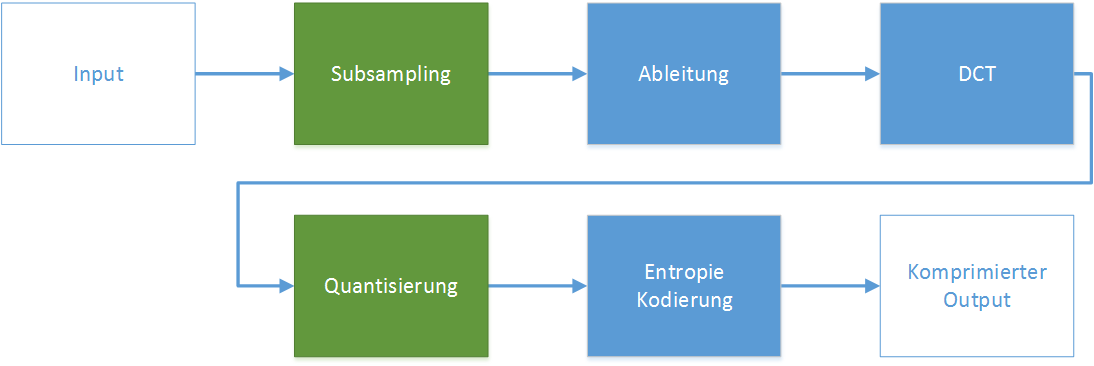
\includegraphics[width=0.8\textwidth,height=6cm,keepaspectratio]{./pictures/konzept/solution1/aufbau.png}
	\caption{Aufbau der Kompression Adaptives Subsampling.}
	\label{konzept:loesung1:aufbau}
\end{figure} 
Die Kompression dieses Verfahrens ist dargestellt im Diagramm der Abbildung \ref{konzept:loesung1:aufbau}. Konzeptionell ähnelt der Algorithmus der JPEG/JFIF Kompression (dargestellt in der Abbildung \ref{state:jpeg:abb}). Im Vergleich zum JPEG/JFIF Standard ist der grösste Unterschied, dass das Eingangssignal vor der Kosinus Transformation abgeleitet wird.

Die Feldlinien ähneln oft harmonischen Halbwellen, welche sich durch wenige Kosinus Funktionen approximieren lassen. Um eine optimale Kompression mit diesem Verfahren zu erreichen, müssen Ringing-Artefakte \cite{wiki:ringing:artefacts} behandelt werden. Sie äussern sich als Oszillationen im dekomprimierten Signal, was das menschliche Auge als störend empfindet. Beispiele für die Ringing-Artefakten von Feldlinien sind im Abschnitt \ref{resultate:loesung1:ringing} zu finden.\\
Es existieren Ansätze die Ringing-Artefakte mit Post-Processing Schritten zu dämpfen: Die simpelste Variante ist, das dekomprimierte Signal zu glätten. Die Glättung kann das Signal verfälschen und ist deshalb nicht die optimale Lösung. In der Bild- und Audioverarbeitung wird nach Post-Processing Filter geforscht, welche die Ringing-Artefakte in der Dekompression vermindern \cite{kaup1998reduction} \cite{park1999postprocessing}. Ein angepasstes Postprocessing wurde im Rahmen dieser Arbeit nicht implementiert.

\subsubsection{Subsampling} \label{konzept:loesung1:subsampling}
Das Subsampling wurde aus der Ist-Kompression \ref{konzept:ist-komprimierung} übernommen. Die Daten werden um den Faktor vier verkleinert, was dazu dient die DCT zu beschleunigen. Eine naive Implementation der DCT weist eine Komplexität von $O(n^2)$ auf. Es wird eine Implementation des FDCT Algorithmus verwendet, welche eine tiefere Komplexität von $O(n log(n))$ besitzt. Der Rechenaufwand ist bei diesem Verfahren trotzdem höher als bei den Verfahren des Adaptiven Subsamplings und der Prädiktiven Kodierung. Falls das Verfahren weiter beschleunigt werden soll, können die Linien in Blöcke unterteilt werden und die DCT pro Block ausführen. Dadurch wird die Komplexität auf $O(n)$ gesenkt. Jedoch ist es wahrscheinlich, dass durch die Unterteilung die Kompressionsrate leidet. Die Approximation mehrere Blöcke des Eingabesignals benötigt schlussendlich mehr Kosinus Funktionen, als die Approximation des gesamten Signals.

\subsubsection{Ableitung}
Das Eingabesignal wird abgeleitet und alle folgenden Transformationen werden auf den Steigungen des Signals ausgeführt. Damit die Transformation umkehrbar ist, muss der Startwert des Signals zusätzlich abgespeichert werden. Die Artefakte, welche das abgeleitete dekomprimierte Signal beinhaltet, sind bei der Feldliniensimulation weniger störend für das menschliche Auge. Die Feldlinie bleibt tendenziell glatt und Artefakte äussern sich meist in veränderten Amplituden, welche erst erkennbar sind, wenn die Originalfeldlinie zum Vergleich bereit steht. Diese Eigenschaft wirkt sich ebenfalls auf die Ringing-Artefakte aus. Die Ableitung hat einen dämpfenden Effekt auf die Ringing-Artefakte.

\subsubsection{Diskrete Kosinus Transformation} \label{konzept:loesung1:kosinus}
Die Diskrete Kosinus Transformation stellt eine endliche Menge von $N$ Datenpunkten als $N$ Kosinus Funktionen dar. Die Werte der DCT-Koeffizienten stellen dar, wie hoch der Anteil einer bestimmten Frequenz im Originalsignal ist. Im optimalen Fall kann ein Signal durch niederfrequente Funktionen approximiert werden. Die hochfrequenten Anteile stellen Detailinformationen dar, die weniger Relevant sind für die Rekonstruktion des Signals als die niederfrequenten Anteile.\\
Es existieren verschiedene Möglichkeiten eine DCT umzusetzen. Hier wurde sich am JPEG/JFIF Standard orientiert, der die DCT-II \eqref{konzept:loesung1:kosinus:formula:fdct} als Vorwärts und die DCT-III \eqref{konzept:loesung1:kosinus:formula:idct} als Rückwärtstransformation verwendet \cite{wallace1992jpeg}. 
\begin{equation} \label{konzept:loesung1:kosinus:formula:fdct}
	X_k = \sum_{n=0}^{N-1}x_n*cos[\frac{\pi}{N}k(n+\frac{1}{2})] \quad k = 0, 1, \ldots, N-1
\end{equation}
\begin{equation} \label{konzept:loesung1:kosinus:formula:idct}
x_n  = \frac{1}{2}X_0 + \sum_{k=1}^{N-1}X_k*cos[\frac{\pi}{N}k(n+\frac{1}{2})] \quad n = 0,1,\ldots,N-1
\end{equation}
$N$ bezeichnet die Länge des Eingabesignals, $x_n$ bezeichnet einen Wert im diskreten Signal und $X_k$ ist der Anteil der Frequenz $k$. Ein Eingabesignal der Länge $N$ resultiert in $N$ Kosinus-Funktionen.

Die DCT transformiert ein periodisches, unendliches Signal. Um ein endliches Signal zu transformieren, wird das Inputsignal konzeptionell an den Rändern gespiegelt. Der Unterschied dieser gewählten Transformationen gegenüber den anderen Verfahren liegt in der Frage, ob bei einer Spiegelung der Randwert wiederholt werden soll. Angenommen ein Signal besteht aus den Daten $a,b,c,d$. Die gewählte Transformation spiegelt das Signal und wiederholt alle Randpunkte: $\ldots,a,b,c,d,d,c,b,a,a,b,\ldots$. Für die Wiederholung der Randpunkte konnte im Bereich der Datenkompression keinen positiven oder negativen Einfluss entdeckt werden. Es wurde deshalb das selbe Verfahren verwendet wie im JPEG/JFIF Standard.

Falls das Signal an den Rändern nicht abflacht, können nach der Quantisierung an den Rändern markante Artefakte auftreten. Ein Beispiel für solche Artefakte ist im Diagramm der Abbildung \ref{resultate:loesung1:dct:artefakte} im Abschnitt \ref{resultate:dct} zu sehen.

\subsubsection{Quantisierung}
In der Visualisierung werden die Feldlinien in drei Typen unterschieden: ''Sonne zu Sonne'', ''Sonne ins Weltall'' und ''Weltall zur Sonne''.  Die ''Sonne zu Sonne'' Feldlinien ähneln harmonischen Halbwellen und brauchen weniger Kosinus Funktionen für eine Approximation als die anderen Typen von Feldlinien. Für die ''Sonne zu Sonne'' Feldlinien werden maximal $35$ DCT Koeffizienten abgelegt, wobei die letzten zehn Koeffizienten kaum noch Einfluss besitzen. Sie werden mit einem hohen Faktor quantisiert, sodass sie im Normalfall ebenfalls Null sind.\\
Die anderen Feldlinien benötigen mehr Koeffizienten für die Dämpfung der Ringing-Artefakte. Bei ihnen liegt das Maximum bei 50 Koeffizienten.

\subsubsection{Entropiekodierung}\label{konzept:loesung1:kodierung}
Um die Entropiekodierung zu verbessern wurden zwei Kodierungen hinzugefügt. Die Längenkodierung reduziert Null-Einträge der Kanäle und die adaptive Genauigkeits-Kodierung reduziert die benötigten Bytes pro Wert eines Kanals.

\textbf{Längenkodierung}\\
Die Quantisierung erlaubt eine maximale Anzahl an Koeffizienten. Ab dem 50 Koeffizient, sind die Werte Null. Die Längenkodierung schneidet den Block von Null-Koeffizienten ab und fügt die Länge des Nicht-Null Blockes hinzu. Alle Längen und alle Blöcke werden zusammen abgespeichert, die Tabelle \ref{konzept:loesung1:entropie:laengenkodierung} verdeutlicht das Konzept. $n_i$ ist die Länge des Nicht-Null-Blocks der Feldlinie $i$ und $x_{i,j}$ ist der $j$ DCT-Koeffizient der Feldlinie $i$.

\begin{table}[!htbp]
	\center
	\begin{tabular}{||c|c|c|c|c||c|c|c}
		\hline
		\multicolumn{8}{|c|}{X Kanäle}\\\hline\hline
		 \multicolumn{5}{||c||}{Block Feldlinie 0} & \multicolumn{3}{c}{\ldots} \\\hline
		$n_0$ &$x_{0,0}$ &$x_{0,1}$ & \ldots & $x_{0,n-1}$ & $n_1$ & $x_{1,0}$ & \ldots\\\hline
	\end{tabular}
	\caption{Beispiel eines abgespeicherten Kanals mit der Längenkodierung.}
	\label{konzept:loesung1:entropie:laengenkodierung}
\end{table}
Um einen Kanal zu Dekodieren, muss die Anzahl an DCT-Koeffizienten $n_i$ gelesen werden und danach Nullen Anfügen, bis die ursprüngliche Länge des Kanals erreicht wurde.

Die Längenkodierung ist effizient, wenn die hochfrequenten DCT-Koeffizienten einen zusammenhängenden Null-Block bilden. Im schlechtesten Fall wäre der letzte DCT-Koeffizient nicht Null. In diesem Fall würde die Längenkodierung nichts abschneiden.\\

\textbf{Adaptive Genauigkeits-Kodierung}\\
Meist reichen sieben Bit Genauigkeit um die quantisierten DCT Koeffizienten darzustellen. Mit der adaptiven Genauigkeits-Kodierung wird ein Minimum an Bytes pro Koeffizient abgespeichert. Die Tabelle \ref{konzept:loesung1:entropie:adaptive} zeigt die Kodierung. Das MSB wird als ''Continue Flag'' verwendet. Wenn es gesetzt ist, gehört das folgende Byte ebenfalls zur Zahl. Die Kodierung führt zu einer Datenreduktion, wenn die Werte im Allgemeinen mit einem Byte dargestellt werden können.

\begin{table}[!htbp]
	\center
	\begin{tabular}{|c|c|c|c||c|c|c|c|}
	\hline
	\multicolumn{8}{|c|}{Byte}\\\hline
	Continue Flag & X & X & X & X & X & X & X \\\hline
	\end{tabular}
	\caption{Aufteilung eines Bytes der adaptiven Genauigkeitskodierung. X sind Nutz-Bits.}
	\label{konzept:loesung1:entropie:adaptive}
\end{table}
\pagebreak

\subsection{Kompressionsverfahren: Prädiktive Kodierung} \label{konzept:prediktiv}
\begin{figure}[!htbp]
	\center
	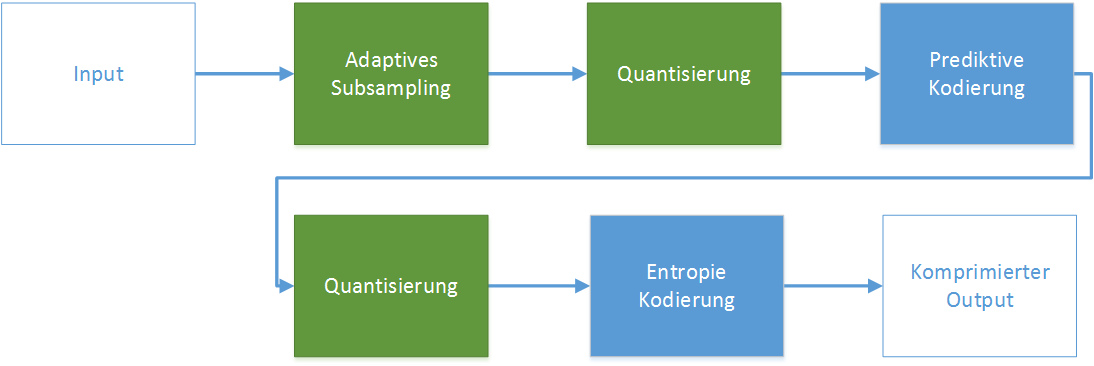
\includegraphics[width=0.8\textwidth,height=6cm,keepaspectratio]{./pictures/konzept/solution2/aufbau.png}
	\caption{Aufbau der Kompressionsverfahren Prädiktive Kodierung.}
	\label{konzept:loesung2:aufbau}
\end{figure}
Die Prädiktive Kodierung ist ein Verfahren, welches in der verlustfreien Kompressionen Anwendung findet. Mittels eines Prädiktors und den bereits kodierten Daten wird eine Vorhersage erstellt für die folgenden Daten erstellt. Die Prädiktive Kodierung speichert ausschliesslich den Vorhersagefehler.

Der Aufbau dieser Kompression ist im Diagramm der Abbildung \ref{konzept:loesung2:aufbau} dargestellt. Im ersten Schritt wird ein Subsampling und eine Quantisierung der Daten durchgeführt. Darauf folgend werden die quantisierten Daten mit einer Prädiktiven Kodierung versehen. Der zweite Quantisierungsschritt löscht unwichtige Vorhersagefehler. 

Das Adaptive Subsampling reduziert die Daten und verändert die Eigenschaften der Kanäle der einzelnen Feldlinien. Stetige Steigungen werden zerstört, ein Beispiel dafür ist im Diagramm der Abbildung \ref{resultate:loesung2:adaptive:channel} im Abschnitt \ref{resultate:loesung2:adaptive} zu finden. Einfache Prädiktoren wie zum Beispiel ein linearer Prädiktor kann auf solche Daten keine zuverlässige Vorhersage treffen und verbessert die Kompressionsrate nicht. Es wurde deshalb der Rekursiver Linearer Prädiktor entwickelt, der auf der Idee der Point Cloud Kompression aus Abschnitt \ref{state:pointcloud} basiert. Die Daten werden in unterschiedlich genauen Approximationen dargestellt. Der Prädiktor benutzt die ungenaue Approximation um eine Vorhersage für die nächst genauere Approximation zu erstellen.

\subsubsection{Adaptives Subsampling und Quantisierung}
Das Adaptive Subsampling der Kompression aus Abschnitt \ref{konzept:loesung0} wurde mit angepassten Parametern übernommen. In dieser Kompression werden $50\%$ mehr Daten übertragen. Die Quantisierung überführt die Punkte in ein diskretes, sphärisches Koordinatensystem. In diesem Koordinatensystem können die Koordinatenachse mit 16 Bit Genauigkeit abgebildet werden, ohne hohe Abweichungen vom Originalpunkt in Kauf zu nehmen.

\subsubsection{Rekursiver Linearer Kodierung}
Der Algorithmus der Rekursiven Linearen Kodierung versucht aus einer ungenauen Approximation die nächst genauere vorherzusagen. Im Diagramm der Abbildung \ref{konzept:loesung2:algorithm:step1} ist der Kodierungsschritt des Algorithmus dargestellt. Es wird angenommen, dass der mittlere Wert des Kanals auf der Strecke zwischen Start- und Endwert liegt. Der Algorithmus wird rekursiv für die zwei Teilstücke des Kanals wiederholt, bis alle Werte zwischen Start- und Endwert des Kanals kodiert wurden. Start und Endwert des Kanals werden nicht kodiert abgespeichert. Die Kodierung der nächsten Rekursionsstufe ist im Diagramm der Abbildung \ref{konzept:loesung2:algorithm:step2} dargestellt.
\begin{figure}[!htbp]
	\center
	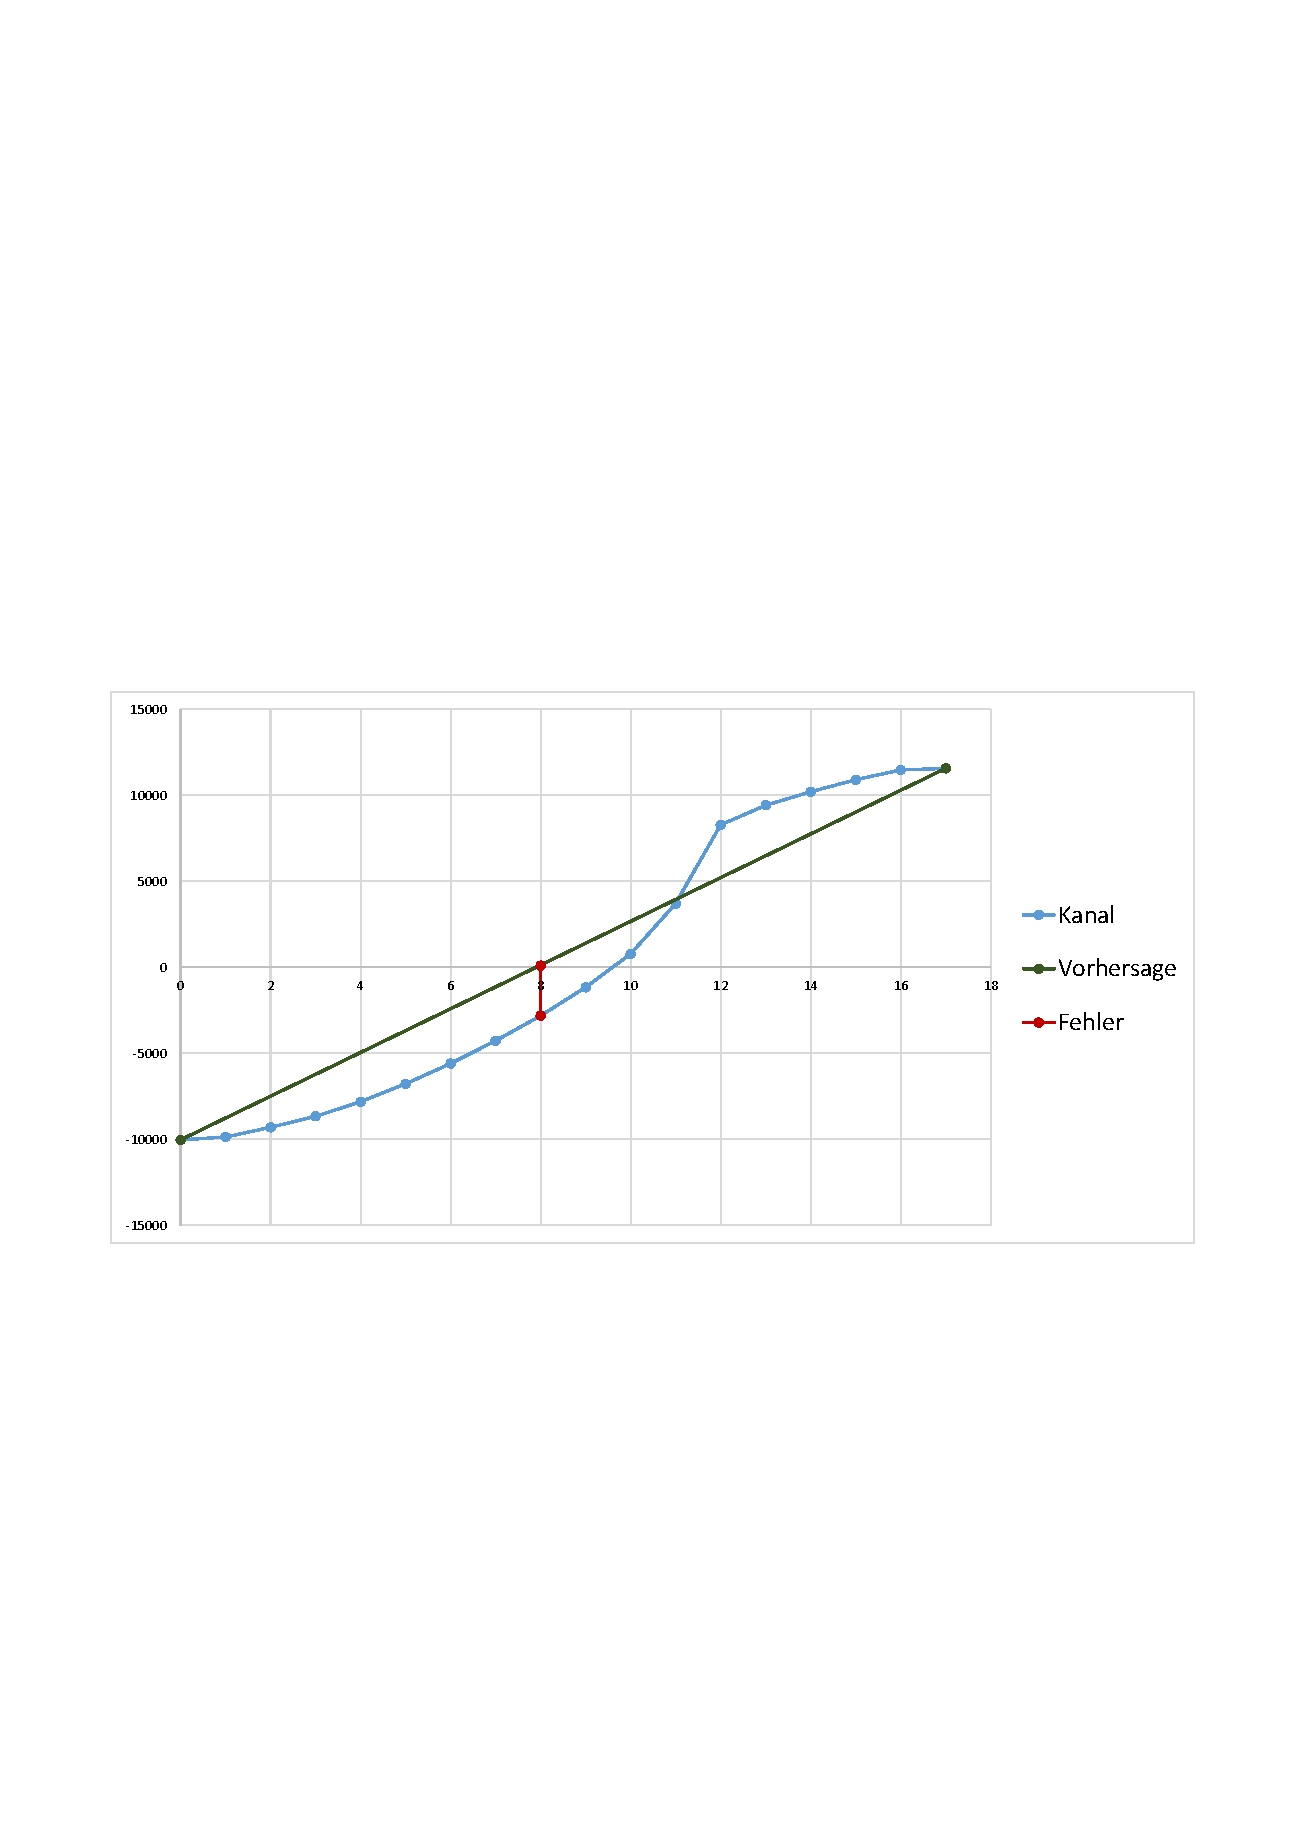
\includegraphics[trim = 1.8cm 10cm 1.8cm 11cm, clip=true, width=1\textwidth,height=8cm,keepaspectratio]{./pictures/konzept/solution2/algorithm_step1.pdf}
	\caption{Erster Schritt der Rekursiver Linearer Kodierung. Zu sehen sind das zu kodierende Signal, die Vorhersage und den Fehler der Vorhersage.}
	\label{konzept:loesung2:algorithm:step1}
\end{figure} 
\begin{figure}[!htbp]
	\center
	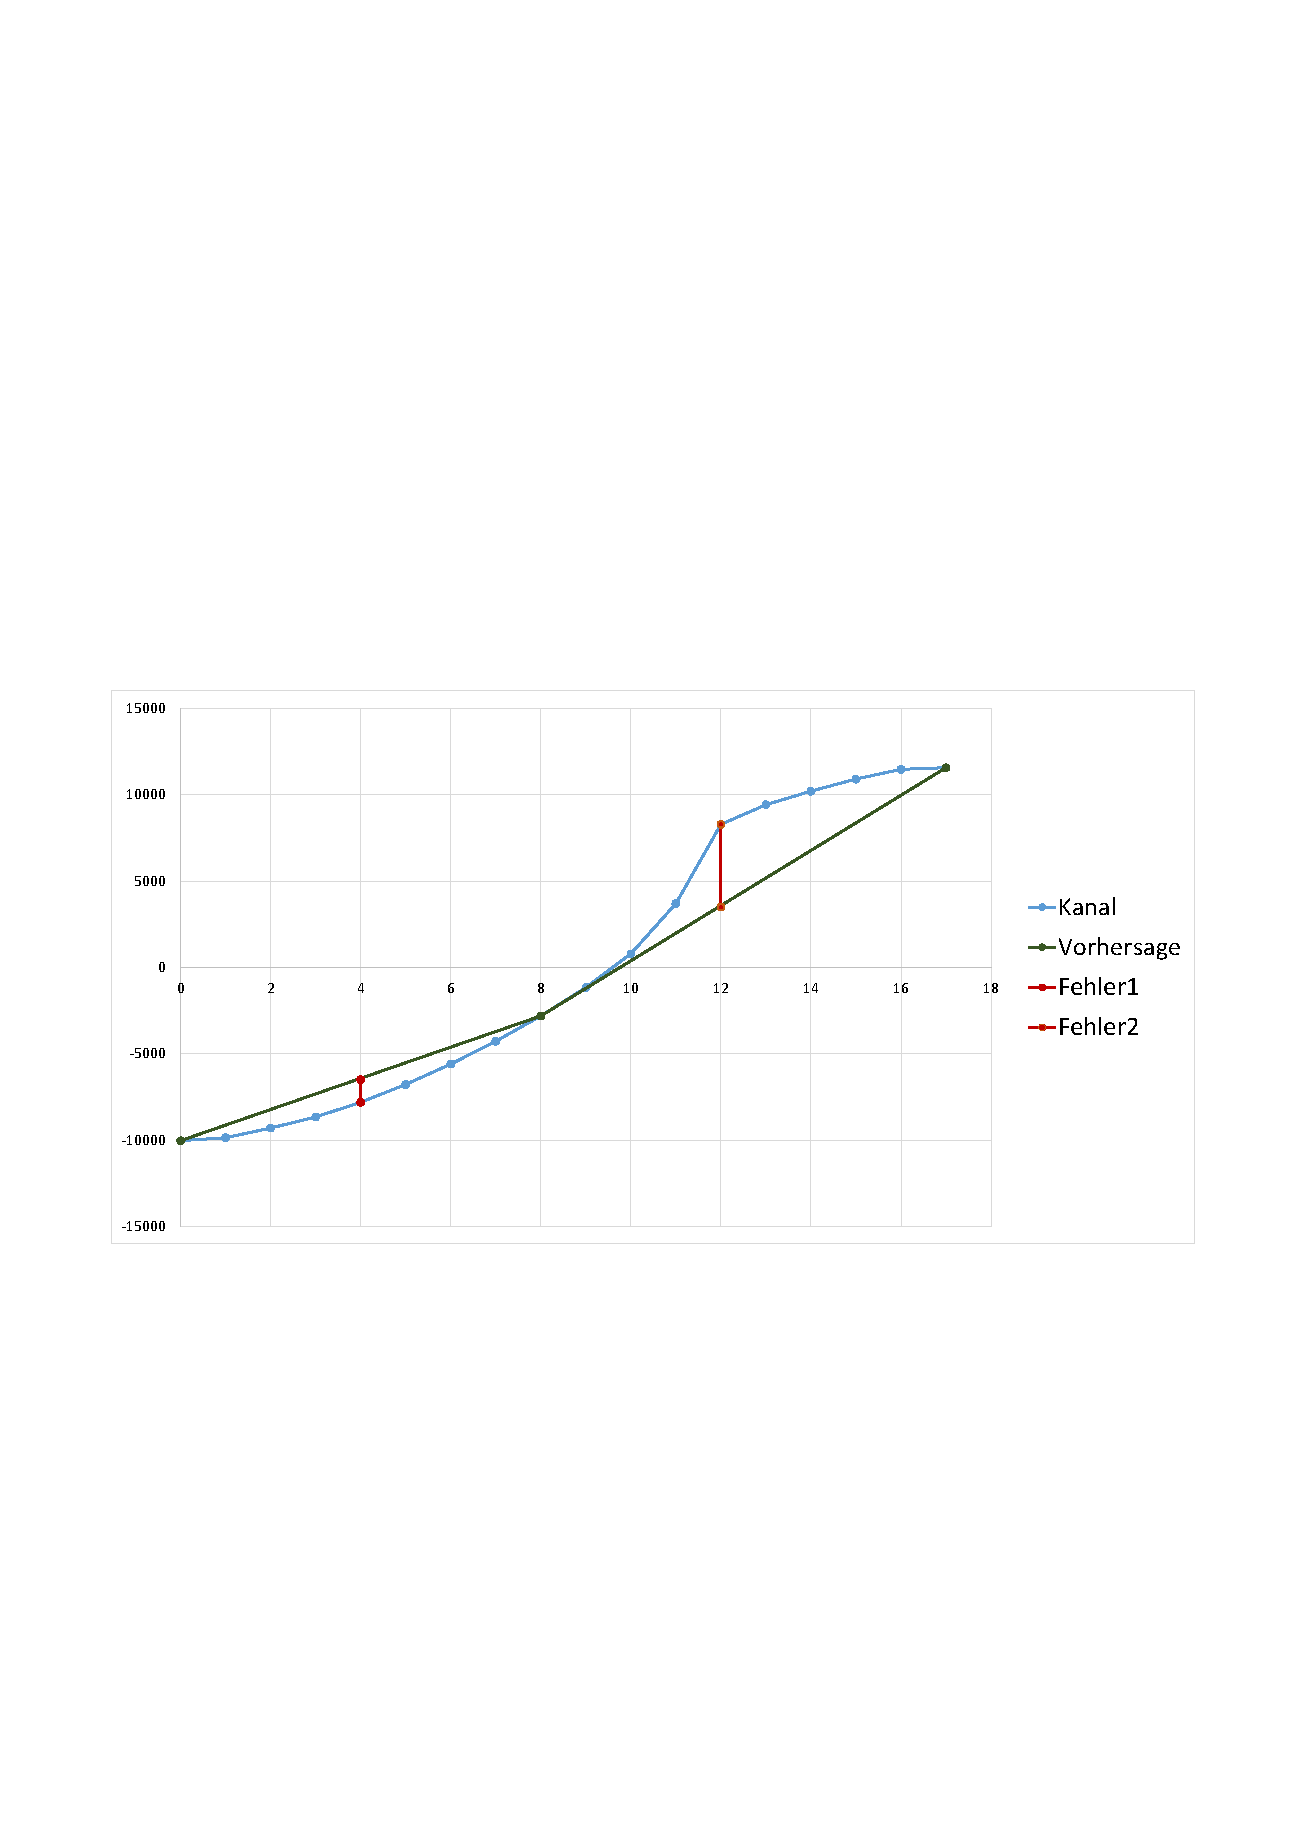
\includegraphics[trim = 1.8cm 10cm 1.8cm 11cm, clip=true,width=1\textwidth,height=8cm,keepaspectratio]{./pictures/konzept/solution2/algorithm_step2.pdf}
	\caption{Zweiter Schritt der Rekursiver Linearer Kodierung. Die Vorhersage beinhaltet nun zwei Strecken.}
	\label{konzept:loesung2:algorithm:step2}
\end{figure} 

\subsubsection{Quantisierung} \label{konzept:loesung2:resudial_quant}
Die Vorhersagefehler der Rekursiven Linearen Kodierung werden von Rekursionsstufe zu Rekursionsstufe kleiner. In der letzten Rekursion werden Detailinformationen kodiert, welche meist nicht relevant sind. Die Vorhersagefehler der ersten Rekursionsstufen werden mit höherer Genauigkeit abgespeichert. Dadurch kann eine hohe Kompressionsrate zu begrenzten Artefakten erreicht werden.

\subsubsection{Entropiekodierung}
Die Vorhersagefehler werden in Breadth-First Ordnung abgespeichert. Der Fehler der Rekursionsstufe 0 wird zuerst abgelegt, gefolgt von den Fehlern der Stufe 1, 2, etc. Die Tabelle \ref{konzept:loesung2:entropie:breath} zeigt den Aufbau. Die Vorhersagefehler der ersten Levels sind grösser, als die der Letzten. Diese Ordnung hilft ähnliche Strukturen beieinander zu halten.

\begin{table}[!htbp]
	\center
	\begin{tabular}{|c||c|c||c|c|c|c||c}
		\hline
		\multicolumn{8}{|c|}{Vorhersagefehler}\\\hline\hline
		 Stufe 0& \multicolumn{2}{|c||}{Stufe 1} & \multicolumn{4}{|c||}{Stufe 2} &\ldots \\\hline
		$Fehler_0$ & $Fehler_1$ &$Fehler_2$ &$Fehler_3$ & $Fehler_4$ & $Fehler_5$ & $Fehler_6$   & \ldots \\\hline
	\end{tabular}
	\caption{Breadth First Ordnung der Vorhersagefehler.}
	\label{konzept:loesung2:entropie:breath}
\end{table}
Die Vorhersagefehler werden mit der Adaptiven Genauigkeitskodierung aus Abschnitt \ref{konzept:loesung1:kodierung} kodiert. Nach der Quantisierung reichen im Allgemeinen 7 Bit Genauigkeit aus, um einen Fehler abzulegen. Die Längenkodierung wurde nicht verwendet.